\documentclass[a4paper,12pt,utf8]{report}

\usepackage{graphicx}
\usepackage[T1]{fontenc}
\usepackage{float}
\usepackage{comment}
\usepackage{hyperref}
\usepackage[english]{babel}

% Useful to show frame around objects :
\usepackage[showframe]{geometry}
% reminder : "showframe" option shows the margins/building rules of the document

% Sticks the footnotes to the bottom of the page, not after the content :
\usepackage[bottom]{footmisc}

% Indent first paragraph after section beginning
\usepackage{indentfirst}

% N.B. this package requires XeLaTeX or LuaTeX :
\usepackage{fontspec}
\usepackage{xunicode}
\setmainfont[Mapping=tex-text]{Linux Libertine O}

% Explicitely set item spacing in lists (as well as top separation with previous textbox) :
\usepackage{enumitem}
\setlist{topsep=5pt,itemsep=5pt}

% Simple command to force the separation of two paragraphs :
\newcommand{\myparspace}{\vspace{\baselineskip}}

\title{Manual for the Prostate3D project}
\author{Thibault de Villèle}
\date{July 2021}

% To make TexLaB shut up on Ubuntu, but also causes the title
% page to disappear. Keeping it here as a reminder.
%\renewcommand\maketitle{}

\begin{document}

\maketitle

% Introduction and how to read this manual :
\chapter{Introduction to the program}\label{text:01_intro}

\begin{comment}
	This section will include :
		- Why this program was created
		- What problems does it tackle / what are its features (very quickly)
		- How to read this manual ?
		- A few definitions
			- notably, the use of certain terms (dataset = 1/multiple 3D image(s))
\end{comment}

\section{What are the main goals of the program ?}\label{text:01_intro:01_goals}
{
	% Why was the program created, what does it do ?

	This program was created during my Master's internship to fit within the project "Visualization, management and processing of high-resolution medical images", done at the University of Montpellier. The work was continued during a small engineering position in 2020/2021. This is the result of those few months of work.

	Its original goal was to provide a simple way to generate high-resolution medical images issued from a \textit{di-SPIM} microscope. To this goal, it had to load a 3D image, downsampled enough to fit within the GPU's memory budget and deform it in order to visualize the resulting image interactively. It then had to allow the user to re-sample a part of the image, and save it to disk for later processing.

	While those tasks were implemented at the end of my internship, we later more features in the following engineering position. We added a real-time volumetric visualization method, allowing to see the sample in three-dimensions interactively. We also added the ability to load grids that would not fit within the memory budget, and downsample them on the fly at loading time in order to visualize bigger acquisitions. We also added the ability to generate the sub-parts of the image in an \guillemotleft~out-of-core~\guillemotright fashion, meaning it does not need to store neither the source image(s) or the resulting image(s) in memory, doing the processing directly from and to the disk.
}

\section{How to read this manual ?}\label{text:01_intro:02_howtoread}
{
	% How to read the manual : in any way you see fit.
	% Chapters have a main purpose, but can be read independently.
	% The code is _will_ change, and is 

	This manual is intended not only for users of the software, but also to provide the next developers of this software with a quick but precise overview of the processing pipeline, and of the underlying code.

	% TODO : add the references to the pipeline and code chapters here
	While chapters \ref{text:01_intro}\footnotemark and \ref{text:01_intro}\footnotemark will be more oriented towards the developers, the more curious users can peruse those parts of the manual in order to gain a better understanding of the inner workings of the code underneath.
	\footnotetext{TODO: change the references to the pipeline and code chapters of this manual.}

	A small note for the developers : this code was made heavily re-done between the internship and the engineering contract to simplify the development of new features, but some parts of it are still a work-in-progress (they will be designated as such in here). If you feel the need to refactor or change large parts of the codebase in order to either specialize or generalize a certain block of code, you're welcome to do it. However, I'd ask you update this documentation to mirror those changes.
}

\section{Glossary}\label{text:01_intro:03_definitions}
{
	For the sake of clarity, here are a few definitions of the words used within this manual, in no particular order :

	\begin{itemize}
		\item \textbf{dataset} : this can be used to design one or multiple images that make up an acquisition
	\end{itemize}
}


% How does the program work in the background :
\chapter{How the program works}\label{text:02_program_flow}

% TOC for ch02 {{{
\begin{comment}
	What will be included in this section :
		- Very brief overview :
			- Open the program
			- Load a grid
			- Visualize it
			- Interact with it
			- Save it/close the program
		- Opening the program :
			- What gets created
			- What can you do right now ?
			- What does the code do in the background ?
		- Loading a grid :
			- What can you load ? (filetypes, types of data) -> for types of data, specify more info will be given in technical doc for the new grid api
			- what parameters can you specify ?
			- How to specify them ?
			- What does the code do in the background ?
		- Visualizing a grid :
			- What can you do ? (different viewing modes and how they work, quickly)
			- How do the things get drawn on screen ?
			- How do the different viewers get controlled ?
			- What does the code do in the background ?
		- Interacting with the grids on screen ?
			- What can you do ?
			- How does it work ?
			- What does the code do in the background ?
		- Generating/saving grids
			- What can you do with this ?
			- How does it work ?
			- What options/parameters can you set ?
			- What does the code do in the background ?
\end{comment}
% }}}

% overview of the system {{{
\section{Overview of the system}\label{text:02_program_flow:01_overview}
{
	%		- Visualize it
	%		- Interact with it
	%		- Save it/close the program

	% intro {{{
	As explained beforehand, this program had a few very simple features, all in order to ease the visualization and management of huge datasets. You can load a big 3D image, visualize it in real-time, and interact with it in a very simple fashion. Afterwards, you can save sub-parts of the grid in a new file. There are of course, some limitations to the kinds of images you can load in memory. Most notably, you can only load a few filetypes into the program. Those are \textsc{Tiff} files, \textsc{OME-Tiff} files, and \textsc{Dim/Ima} files.\par
	Let us go through the program as it is supposed to be used, steop by step.\par\myparspace
	% }}}

	% opening program {{{
	\subsubsection*{Opening the program}
	{
		% figure : program ui start {{{
		\begin{figure}[h]
			\label{figure:program_ui_00}
			\centering
			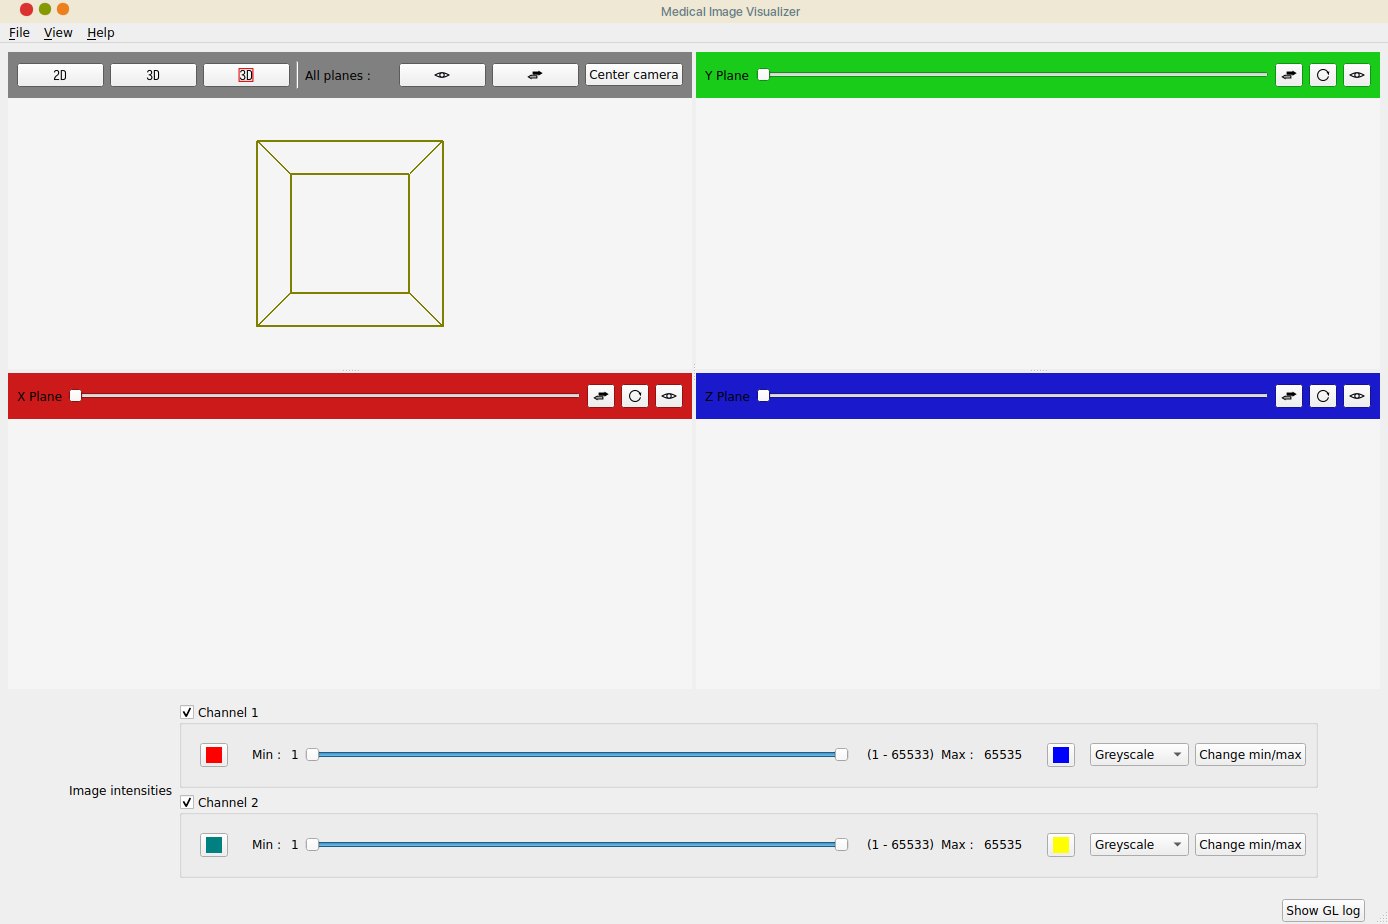
\includegraphics[width=.75\textwidth]{img/program_00.png}
			\caption{The default interface of the program.}
		\end{figure}\par
		% }}}
		% opening : 4 windows & their headers {{{
		Upon opening the program (as illustrated in figure \ref{figure:program_ui_00}), you'll be greeted by four distinct windows directly in the center of the program. The upper left-hand window allows to see the loaded images in three dimensions, and by default only shows an olive-colored wireframe cube. The upper right-hand window will show the contents present at the position of the XZ plane, once an image is loaded. The bottom left-hand and right-hand windows show the contents of the YZ and XY planes respectively, once an image is loaded.\par
		At the top of those four \guillemotleft{}~visualization windows~\guillemotright{}, you'll find a header which can control some of the aspects of the window they're attached to.\par\myparspace
		% }}}
		% bottom : sliders and colors {{{
		The bottom quarter of the program's window contains two group boxes, each containing a range slider (containing two handles), two colored buttons, a drop-down menu and a button labelled \guillemotleft{}~Change min/max~\guillemotright{}. We'll explain what those do in just a moment. And finally, a \guillemotleft{}~Open GL log~\guillemotright{}~ button which is the OpenGL log (intended for debugging).\par
		\myparspace
		% }}}
	}
	% }}}

	% loading a grid {{{
	\subsubsection*{Loading a grid}
	{
	% warning : api in shift {{{
	\textit{Note} : this section of the program contains code that is subject to change, due to an architectural change of the internal grid representation. See section \ref{text:03_software_components:01_image_representation:03_migration} and section \ref{text:03_software_components:01_image_representation:02_modern_grid} for more information.\par\myparspace
	% }}}
	% figure : program file loading dialog {{{
	\begin{figure}[h]
		\centering\label{figure:program_ui_01}
		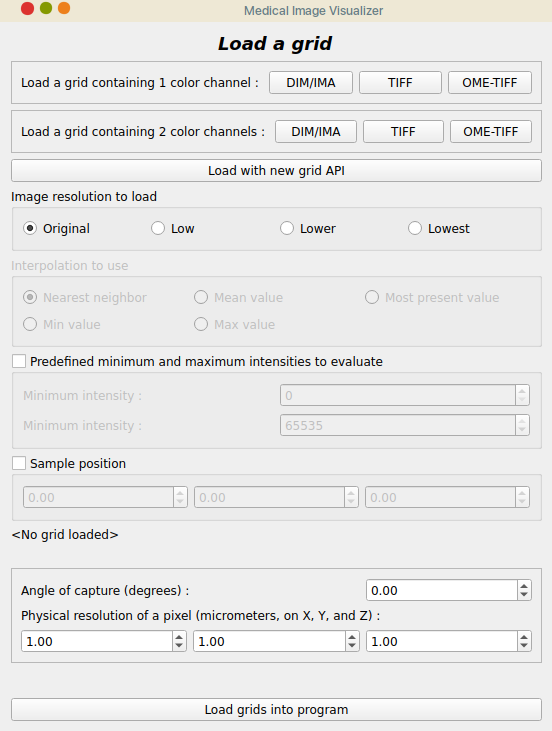
\includegraphics[width=.6\textwidth]{img/program_01.png}
		\caption{Image loading dialog}
	\end{figure}\par
	% }}}
	% intro to loading {{{
	Once the program is open, the user can load a grid by either pressing the \textit{File > Open images} menu item, or by pressing \texttt{\textit{Ctrl+O}}. From there, the user is greeted with a new window, where they can choose the type of file to load.\par
	The different buttons laid out at the top of the window all serve a slightly different purpose. The first group of buttons (in the top frame) allow the user to load a greyscale dataset from disk, using one of the formats available at its disposal. Selecting a filetype and attempting to load another filetype will result in an error and no grid being loaded.
	The next group of buttons tries to load a 2-channel dataset from disk, with the same modalities as before. And the last button is currently only a test of a new implementation of the internal grid representation, and can only load two \guillemotleft{}~stacks~\guillemotright{}~of files saved as \texttt{Tiff}.\par\myparspace
	% }}}
	% list of parameters in the dialog {{{
	Within this window (shown in figure \ref{figure:program_ui_01}), the user can specify a few different parameters. The user-specifiable parameters start from below the \guillemotleft{}~\textit{Load with new grid API}~\guillemotright{}~button. From top to bottom, those are :
	\begin{itemize}
		\item \textit{the resolution to load} : this specifies the amount of downsampling to apply to the image. By default, the grid is loaded in full resolution. And then, the grids are loaded at $\frac{1}{8}$-th, $\frac{1}{64}$-th, or $\frac{1}{512}$-th resolution, by pressing the \textit{Low}, \textit{Lower}, and \textit{Lowest} buttons respectively (each level divides the resolution on each axis by 2).
		\item \textit{the interpolation to apply} : specifies the interpolation to apply when downsampling the grid on load. The user can specify any option amongst \textit{Nearest Neighbor}, \textit{Mean value}, \textit{Most present value}, \textit{Min value}, and \textit{Max value}.
		\item \textit{the range of values to evaluate} : if the user already knows the range of \guillemotleft{}~interesting values~\guillemotright{}~to evaluate, it can be specified here and the visualization pipeline will take it into account when setting the range of values visible.
		\item \textit{sample position} : this allows the user to specify an approximate offset of the dataset from the origin. Completely optional.
		\item \textit{angle of capture} : this parameter is for \textit{di-SPIM} captures that have not yet been resampled in world space. This value (expressed in degrees) will be the angle of capture of the microscope camera from the normal to the sample.
		\item \textit{physical resolution of a pixel} : expressed in micrometers, this will define the size of a voxel in the loaded grid.
	\end{itemize}\par
	% }}}
	% parameters can be left blank, no errors = dimensions in label {{{
	All of those parameters can be specified by the user, or filled automatically if the filetype has additionnal metadata representing those variables. Do note that upon specifying a set of files to load, the window may freeze for a couple of seconds as it parses the stack of filenames. The user will know the grid has been properly parsed without errors if the dimensions of the grid appear in the label in the middle of the window, which currently says \guillemotleft{}~no grid loaded~\guillemotright{}.\par\myparspace
	% }}}
	}
	% }}}

	% visualization & interaction w/ grids {{{
	\subsubsection{Visualizing and interacting with the loaded image}
	{
		After the user specified the grid to load as well as its parameters, the data contained in the grid is processed and uploaded to the GPU. A quick processing step (that might freeze the window) later, and the grid is ready to be visualized.\par
		The controls for the visualization are located at the bottom of the grid, and allow to specify multiple parameters : the range of values to display, as well as the color scale to use.
	}
	% }}}

	% grid generation {{{
	\subsubsection{Generate and save the grid}
	{
		%
	}
	% }}}

}
% }}}

% program flow, object lifetime in the program {{{
\section{Program lifetime}\label{text:02_program_flow:02_object_lifetime}
{
	This section is mainly aimed at developers. It will go through the same program workflow, and detail what resources are created, how they are created and how to find them in the code.

	% opening the program {{{
	\subsubsection{Opening the program}
	{
		%
	}
	% }}}

	% loading grids {{{
	\subsubsection{Loading the grid}
	{
		%
	}
	% }}}

	% visualization / interaction {{{
	\subsubsection{Visualizing and interacting with the loaded image}
	{
		The visualization pipeline is written to be compliant with OpenGL 3.2. This choice was made to ensure a wider portion of the currently-used graphics hardware could run the program. Most notably, the computers at the IGF were not updated to the latest graphics driver (to ensure compatibility with a proprietary software they use), forcing us to downgrade the OpenGL version required to be 3.2.\par
		Most of the program \textit{should} work with OpenGL 2.0, as long as some extensions are required when the program starts (most notably, vertex array objects and buffers should be present). See \textit{Qt}'s and OpenGL's documentation on how to get the available extensions on a system at runtime, and read on to see the technical requirements of the program.

		% should talk about :
		% tetra mesh, range of values init in the scene classes, color scales (that are not in use yet, still
		% uses the ones in the grid !!!), and then the upload of tet mesh to the GPU
	}
	% }}}

	% grid generation {{{
	\subsubsection{Generate and save the grid}
	{
		%
	}
	% }}}
}
% }}}

% Vim modeline, do not touch !
% vim : set breakindentopt=shift\:2 :

% What components are there, how do they interact (...) :
\chapter{Software components}\label{text:03_software_components}

% Outline of the file {{{
\begin{comment}
	What are the major software components of the program, what is(are) their role(s)
		- Image representation in memory
			- Old way : DiscreteGrid
			- New way : Grid<ImageBackendImpl>
		- Visualization primitives
			- Viewers : 3D and 2D
			- Scene
			- The different components of the scene, more detailed
		- Generation primitives
		- Tasks / multi-threaded stuff
		- General purpose / other things that didn't fit into above
\end{comment}
% }}}

% Quick intro about the general organisation of tasks and files ... etc {{{
This section is aimed more at developers which will take over this project and extend it. It describes in detail the different software components in the program, as they are at the end of my engineering contract.

\vspace{\baselineskip}

However, do note that \textit{this is not a precise documentation of every function and class of the program}, this is simply an enumeration of the different concepts present in the code, where to find them and how they are used within the context of the program. For a complete documentation, please see the code or the \textsc{Doxygen} file for a more detailed listing of available classes and functions.

\vspace{\baselineskip}

For every concept and class described here, there will be a path allowing you to find them in the code. This path is always relative to the root of the git repository that was cloned in order to get this code. In addition, there will be additional information present here about the state of the concepts/classes (if they are in-progress or not).
% }}}

% Section 1 : image representation {{{
\section{Internal image representation}\label{text:03_software_components:01_image_representation}
{
	% Intro to the internal image representation {{{
	\textit{N.B.} : Throughout this part, I'll use the terms \textit{grid} and \textit{image} interchangeably. This is only because we consider the three-dimensional images to be a regularly sampled 3D grid, of resolution equal to the image resolution and with additional metadata which we can garner either from the image files themselves, or from user input.
	% TODO : Maybe put the paragraph above in a 'quote' block ?
	% Meaning, grey background, font a bit smaller and italic all the way through

	\vspace{\baselineskip}

	Due to a slightly chaotic organization on my part regarding the different software components, there are actually two ways to represent grids within the program. Those two implementations both serve the same purpose : to deliver a way to get information about the grid easily from within the code. However, that's where the similarities end. The two grids differ quite a bit in their implementation, but the interoperability of the two function interfaces is quite good.

	\vspace{\baselineskip}

	I'll go over the legacy way of loading and addressing grids first. I'll explain what I did and why I did it before going over the recommended way of loading grids. I'll also explain why this implementation is better, even if it does mean having a bit more trouble to write the code to access the grid's data.
	% }}}

	% DiscreteGrid explanation {{{
	\subsection{Legacy grid representation : \texttt{DiscreteGrid}}\label{text:03_software_components:01_image_representation:01_legacy_discretegrid}
	{
		% Where are the files within the git repository ?
		% What does the class do ?
		% Where/How is it used ?
		% What doesn't it do ?
		% Why is it deprecated ?

		\texttt{DiscreteGrid} is the legacy implementation of a voxel grid. It was developed during the last few weeks of the internship, and the first couple of weeks of the engineering contract. You can find it in the repository under the \texttt{grid/} folder. The header files are under \texttt{grid/include/} while the implementation is under \texttt{grid/src/}. This was the main way to represent a grid in memory until a new and admittedly better implementation came along.\par

		\vspace{\baselineskip}

		This class is able to represent a dense\footnote{non-sparse}, regularly sampled three dimensional voxel grid. This voxel grid has a few different attributes which we can gather and modify from the images loaded :\begin{itemize}
			\item the grid's resolution,
			\item the voxel sizes of the grid,
			\item the transform to go to and from the image space
			\item the surrounding bounding box (in image space)
		\end{itemize}\par

		\vspace{\baselineskip}

		Those attributes were not always set based on the information found in the image files It was a first naive implementation of a voxel grid, and as such it has a few pros and cons to be aware of :\begin{itemize}
			\item the grid can only load single-channel data (no two channel data, no RGB \ldots{})
			\item the \texttt{DiscreteGrid} class is actually a virtual class. The concrete implementations have different uses and are defined as :\begin{itemize}
					\item input grids (defined by the \texttt{InputGrid} class). This represents the grids taken from on-disk 3D images, and its data cannot be modified. All of its data can either be \textit{entirely} loaded in memory, or \textit{entirely} left on-disk (a small cache of recently accessed slices is kept)
					\item output grids (defined by the \texttt{OutputGrid} class). This represents grids generated during the runtime of the program, and cannot have on-disk images as an input. All its data \textit{must} be in-memory.
			\end{itemize}
			\item the grid provides access to limited information about the grid (expressed in the list above)
			\item we can transform point to and from the image's initial space
			\item the class can store different types and sizes of data (signed or unsigned, 8/16/32 bits \ldots{}). This type is also used in the classes that read the data from and write the data to the disk.
		\end{itemize}

		\vspace{\baselineskip}

		This particular structure was made with the idea that the reading and writing logic for the different file types was uncorrelated with the grid, and could be put in a separate set of classes : the \texttt{GenericGridReader} and \texttt{GenericGridWriter} classes respectively. Over time, the grid and reader/writer classes were becoming so similar that most of the data was effectively duplicated.

		As a first draft of a grid representation, it did the job pretty well. However, some severe limitations quickly arose. Most importantly, the clear separation between input and output grids which was thought to be very important at the beginning proved to be more of a hindrance than anything else (as a result, the code implementing the input and output grids was slowly upstreamed into the \texttt{DiscreteGrid} class over time).\par

		\vspace{\baselineskip}

		Additionally, the fact that changing the grid input type requires a recompilation of the program to be updated is not optimal not only for the user of the program which can thus only load a certain type of data, but also for the developer which would be forced to reimplement the whole thing for different types (yes, the architecture was \textit{that} bad).\par

		As such, it became clear that a new implementation of a grid was necessary not only for the ease of use it would provide, but also for the developers of the project.
	}
	% }}}

	% Modern `Grid` class {{{
	\subsection{Modern grid representation : \texttt{Grid}}\label{text:03_software_components:01_image_representation:02_modern_grid}
	{
		% Where are the files within the git repository ?
		% What does the class do ?
		% Where/How is it used ?
		% HOW DOES IT WORK ? (explain the template functions and the explicit tagging system for them)
		% What doesn't it do ?
		% Why is it better than DiscreteGrid ?
		% How can we extend it ?

		To replace the old \texttt{DiscreteGrid} implementation, a new grid representation was developed : \texttt{Grid}. The files for this implementation can be found in the repository under the \texttt{image} folder, more specifically in the \texttt{api}, \texttt{tiff} and \texttt{transform} folders.\par

		\vspace{\baselineskip}

		% list of features {{{
		This new implementation of the voxel grid is still a bit of a work in progress on some fronts. This refactoring of the internal grid representation had a few goals over the existing solution :\begin{itemize}
			\item allow to load multiple types and sizes of data using the same class and function interface
			\item consolidate the different (input/output) grid types into a single class since their separation is not necessary
			\item have the reading/writing logic directly set into the class itself, since it is an integral part of the grid
			\item allow for multi-channel data (the current implementation actually supports any number of channels, even though it's mostly RGB data that will be loaded)
		\end{itemize}
		%}}}

		% we chose pimpl {{{
		There were a myriad of ways to implement an interface with all those goals. The most popular way to implement such a set of features uses template meta-programming to perform type erasure on the image struct. It is quite common to see this in widely used C++ image toolkits such as \textsc{Vtk} or \textsc{Itk}. However, this method requires a deep and intrinsic knowledge of how templates work, and makes the code a bit less readable. As such, the one chosen here follows the \texttt{pImpl}\footnote{\href{https://en.cppreference.com/w/cpp/language/pimpl}{https://en.cppreference.com/w/cpp/language/pimpl}} idiom : it hides the implementation details of a class behind a private pointer. It is what's used for most of \textsc{Qt}'s widgets. \par

		\myparspace
		% }}}

		% pimpl is flexible for image formats/types/sizes {{{
		This flexibility in the implementation details or \guillemotleft{}~backend~\guillemotright{}~of the grid allows us to effectively make as many implementations as necessary, and choose the correct one at runtime. As an added bonus, it provides the developers of the program with a single, non-templated interface which they can use to access a multitude of different image formats, and data types and sizes.\par

		\myparspace
		% }}}

		% more details about interaction grid/image_backend {{{
		The \texttt{Grid} class is a well-defined, concrete type that can only be constructed using a valid pointer to a previously-allocated \texttt{ImageBackendImpl}. Whenever a function is called on a \texttt{Grid} object, the class calls a similar function in the image backend, allowing to define the proper behaviour dynamically.\par
		The \texttt{ImageBackendImpl} class is a virtual-only class which serves as an interface for the different backends that can be implemented. This allows to write a specialized class for each image type that we want to support. Let's study the implementation details of a particular file type : the \texttt{Tiff} file type.
		% }}}

		\subsubsection{Case study : the \texttt{Tiff} image backend}
		{
			% How it's structured - TIFF {{{
			\texttt{Tiff} is a popular file format that allows the storage of one or multiple 2D images. It does this by defining a \textit{directory} type, which is a fully documented subsection of the file containing the image data of a single image. The \texttt{Tiff} specification\footnote{\href{https://www.adobe.io/content/dam/udp/en/open/standards/tiff/TIFF6.pdf}{\texttt{Tiff} specification, v6.0 (adobe.io)}} also states that data can be encoded as signed integers, unsigned integers, floating-point or complex numbers with sizes between 1 and 4 bytes per sample. There can be from 1 to 5 samples per pixel\footnote{RGB data along with 2 additional samples usually reserved for raw and premultiplied alpha}.
			% }}}

			% Many possibilities, so implemented a base class and template spacializations {{{
			With such a breadth of possibilities for the \texttt{Tiff} format, we have to provide an implementation which will cover most of usual configurations of data that can be saved in a \texttt{Tiff} file. As such, a \texttt{TIFFBackendImpl} class was implemented, which inherits the \texttt{ImageBackendImpl} class. This is the base class for our \texttt{Tiff} implementation.\par
			To tackle most possible configurations of \texttt{Tiff} files, this class is then derived once more into a templated class : \texttt{TIFFBackendDetail<pixel\_t>}. This class's template argument, \texttt{pixel\_t} is the type of data contained within the file. This is the lowest-level class in our hierarchy, and this is also the once which implements the \guillemotleft{}~low-level~\guillemotright{} logic to handle \texttt{Tiff} files.\par
			% }}}

			\myparspace

			Due to the ability of C++ to perform runtime polymorphism, we can specify that the \texttt{Grid} class accepts a pointer of type \texttt{ImageBackendImpl} and specify the right type of backend to create at runtime. Here's a short example :

			% Code listing : grid creation example {{{
\begin{lstlisting}[style=cppbasicstyle, caption={Creating a grid}]
std::vector<std::string> filenames = /* ask user ... */ 
// Assume the internal data type is 'pixel_type' :
Grid::Ptr grid = Grid::createGrid(
 TIFFBackendDetail<pixel_type>::createBackend(filenames)
);
// Grid is created, and will sample the user-given files
\end{lstlisting}
			% }}}

			If any problem occurs during the file parsing, the error is propagated up through the call stack and can be caught by the caller of the \texttt{Grid::createGrid()} function. This allows the user to know the source of the problem, and rectify it.
		}
		\myparspace

		Once the grid and corresponding backend is created, we have to be able to give access to the data contained in the source image files.

		\subsubsection{Accessing the grid}
		{
			% C++ being a real pain about templates+runtime polymorphism causes issues {{{
			Due to the wide variety of possible data types being loaded into memory, a template function is essential. However, C++ does not allow to specify templated function definitions as virtual when the base class itself is not templated. Due to this language limitation, we cannot directly access the data contained in the underlying concrete implementations (such as \texttt{TIFFBackendDetail<>}). Furthermore, the base class of \texttt{ImageBackendImpl} carries no information about the internal fundamental type used by the concrete implementation.\par
			% }}}

			% Impl of the read functions : call hierarchy {{{
			To circumvent this limitation, we implemented the pixel read functions on multiple levels :\begin{enumerate}
				\item the \texttt{Grid} class contains a templated member function to read pixels, lines or entire slices of the dataset.
				\item the \texttt{ImageBackendImpl} base class contains a templated equivalent of the \texttt{Grid} functions which calls an internal function : \texttt{internal\_readRegion()} which is \textit{not} templated
				\item since the \texttt{internal\_readRegion()} function is not templated, it can be declared as virtual and thus can be overridden in derived classes.
			\end{enumerate}\par
			The \texttt{internal\_readRegion()} functions do however need to be specialized for each type to support (in our case, nearly all fundamental arithmetic types from the STL). This would normally cause an overload problem, where many functions are defined with a different signature. However, we can avoid this trouble entirely by relying on an explicit tagging system by providing a templated, unused object in the function definition which allows C++'s argument-dependant lookup to find the right signature for a given call. Here's an example of the definition of such functions :

			\begin{lstlisting}[style=cppbasicstyle, caption={Example of the explicit tagging system in use}]
// When called from a 'std::uint8_t' template :
void internal_readRegion(tag<std::uint8_t> tag, ... );
// When called from a 'std::uint16_t' template :
void internal_readRegion(tag<std::uint16_t> tag, ... );
// When called from a 'double' template :
void internal_readRegion(tag<double> tag, ... );
			\end{lstlisting}
			% }}}
		}

		% Why better than DiscreteGrid ? {{{
		This architecture offers some obvious benefits over the legacy implementation given by the \texttt{DiscreteGrid} class. The most obvious one being the flexibility given to load images of different internal types at runtime.
		% }}}
	}
	% }}}

	% Migration between the two : progress {{{
	\subsection{Code migration}\label{text:03_software_components:01_image_representation:03_migration}
	{
		% Explain what parts are not et migrated to the new code
		% How can we migrate them ?
	}
	% }}}
}
% }}}

% Section 2 : Visualization components {{{
\section{Visualization of different components}\label{text:03_software_components:02_visualization}
{
	%
}
% }}}

% Section 3 : generation primitives {{{
\section{Generation primitives}\label{text:03_software_components:03_generation_primitives}
{
	%
}
% }}}

% Section 4 : about multi-threading {{{
\section{Tasks and multi-threading}\label{text:03_software_components:04_tasks}
{
	%
}
% }}}

% Section 5 : other stuff {{{
\section{Other structures}\label{text:03_software_components:05_other}
{
	%
}
% }}}

% Vim modeline, do not touch !
% vim: set breakindentopt=shift\:2 :

% How do I do X ? (F.A.Q.-like section for both users and developers)
\chapter{How do I ...}

\begin{comment}
	What will be included in this chapter :
		- User-facing stuff :
			- how to open/use the program, in general
				- use the help guide
				- say what can be loaded
				- describe interactions
				- describe viewing modes
				- describe output data (generation)
			- how to load data
				- what kind of filetypes are supported
				- what are some caveats/'gotchas' of the program
				- some of the options within the loading dialog
				- what the loading dialog should result in
			- how to generate grids
				- what the intent was to do something like this
				- how to use it
				- specify the process is blocking !!! no progressbar
				- what can be done with this
		- Dev-facing stuff :
				- How do I compile the program ?
					- The included third-party libraries
						- How to include them in the directory structure and in the compilation process
					- Compile the libs with the ./third_party/compile.{ps/sh} utilities
					- Use CMake
					- Learn about CMake flags !!!
				- How do I debug something ? -- Graphical
					- use renderdoc ! wonderful
				- How do I debug something ? -- Code
					- Learn a debugger (Qt's one is good)
					- Most code is documented, use this as a first step
					- Be warned, some things are multi-threaded so printf() might not always result in a useful thing.
				- How do I draw something ? [ NEEDED ??? ]
					- make sure context is bound
					- specify commands with an instance of QOpenGLFunctions (Scene, or within a drawable class)
					- some words about the composition of the widget, that all should be drawn and that Qt will do its stuff later
					- ping the reader back to the documentation of the pipeline
\end{comment}


\end{document}

